%/*****************************************************************************
% * CLI Instructions
%/*****************************************************************************

\documentclass[12pt]{article}
\usepackage{float}
\usepackage{graphicx}
\usepackage[margin=1in]{geometry}

\graphicspath{{images/}}

\usepackage[utf8]{inputenc}
\usepackage[english]{babel}
\usepackage[parfill]{parskip}
\usepackage{datetime}
\usepackage{hyperref}
\hypersetup{
	colorlinks=true,
	urlcolor=blue,
  }
\urlstyle{same}
\usepackage{subcaption} 
\usepackage{dirtytalk}
\usepackage{multirow}
\usepackage{booktabs}


\usepackage{fancyhdr}
\pagestyle{fancy}
\fancyhf{}
\rhead{WindNinja Command Line Interface Instructions}
\cfoot{\thepage}

\newcommand\vn{3.6.0}

\begin{document}
\begin{titlepage}
    \centering
    {\Huge
       Instructions for using WindNinja's command line interface (CLI)
    }    
    \vfill
    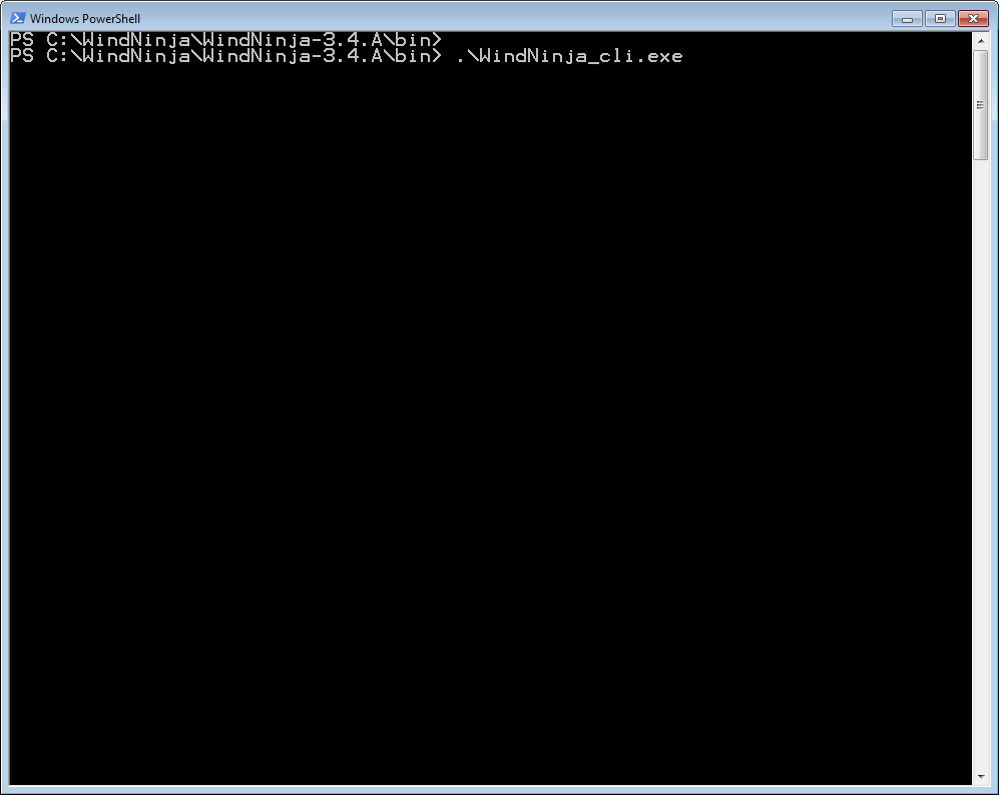
\includegraphics[scale=0.75]{cli-0}
    \vfill
  	{\Huge
	  3/25/2020 %Date Last Edited
  	}
    \vfill
\end{titlepage}
\section*{Introduction}
To allow WindNinja to be used more easily by other programs or through scripting, a command line interface (CLI) has been developed.  Programmers should find this very useful, however, most WindNinja users (fire managers and fire modelers) will not use the CLI.  This short paper gives a description of how to use the CLI.  It assumes that you have some experience running programs from the command line (terminal).

The WindNinja cli is provided as a separate executable called “WindNinja\_cli.exe”.  This executable comes with the normal installation of WindNinja for the Windows operating system (in the “bin” directory).  It is also possible to run WindNinja on GNU/Linux.  Users interested in the Linux version should %contact Jason Forthofer at jaforthofer@fs.fed.us.  
visit the \href{https://github.com/firelab/github}{WindNinja development website}. 
The CLI executable is dependent on all of the dynamic link libraries provided in the “bin” directory (libcurl.dll, gdal18.dll, etc.) except the Qt libraries “Qt4Core4.dll” and “QtGui4.dll” (used only in the gui version).

%I don't think this needs to be done anymore
%\section*{Setting the Environment}
%To do a run from the terminal, it is recommended that you add the WindNinja bin directory to the “Path” environment variable.  This can be done on some Windows systems by doing this:
%\begin{enumerate}
%\item Right-click \textbf{My Computer} and select \textbf{Properties}.
%\item Select the \textbf{Environment} page.
%\item In the \textbf{System Variables} area, highlight the current \say{Path} and click \textbf{Edit}. 
%\item Add the new path \textit{to the end} in the format \texttt{VALUE1;VALUE2;} \textbf{Be sure you don't delete any of the other paths!!} For example, if WindNinja 2.1.0 was installed in the default directory, add this to the end of the current path: \texttt{;C:\textbackslash WindNinja\textbackslash WindNinja-2.1.0\textbackslash bin}
%\item Click \textbf{OK} to close all of the windows you have opened.
%\item The changes take effect immediately, however if you had a terminal open before you made these changes, you should close it and reopen one for the new settings to take effect.
%\end{enumerate}

\section*{Starting A Run}
A cli run must be started from a terminal (or “spawned” or something equivalent when called from another program).  You type the name of the cli executable (“WindNinja\_cli.exe”) and then options (arguments) to specify information about the run.  The options can either be specified directly from the terminal, by using a configuration file, or some combination of these.  To use the terminal, just type the executable followed by the options and associated values.  To use a configuration file, just type the name of the executable followed by the name of the configuration file (absolute or relative path from the location of the executable file).  %To use a response file, type the name of the executable followed by “@name” where “name” is the name of the response file.  All of these methods of starting a run with the cli are described in more detail below.

\section*{Available Options}
The available options with descriptions can be viewed by typing:
\begin{itemize}
\item[]\texttt{WindNinja\_cli.exe}
\end{itemize}
(note that it is optional to add the file extension “.exe” to “WindNinja\_cli”)
A list of the available options should be shown and look similar to this:
\begin{figure}[H]
	\centering
	\label{}
	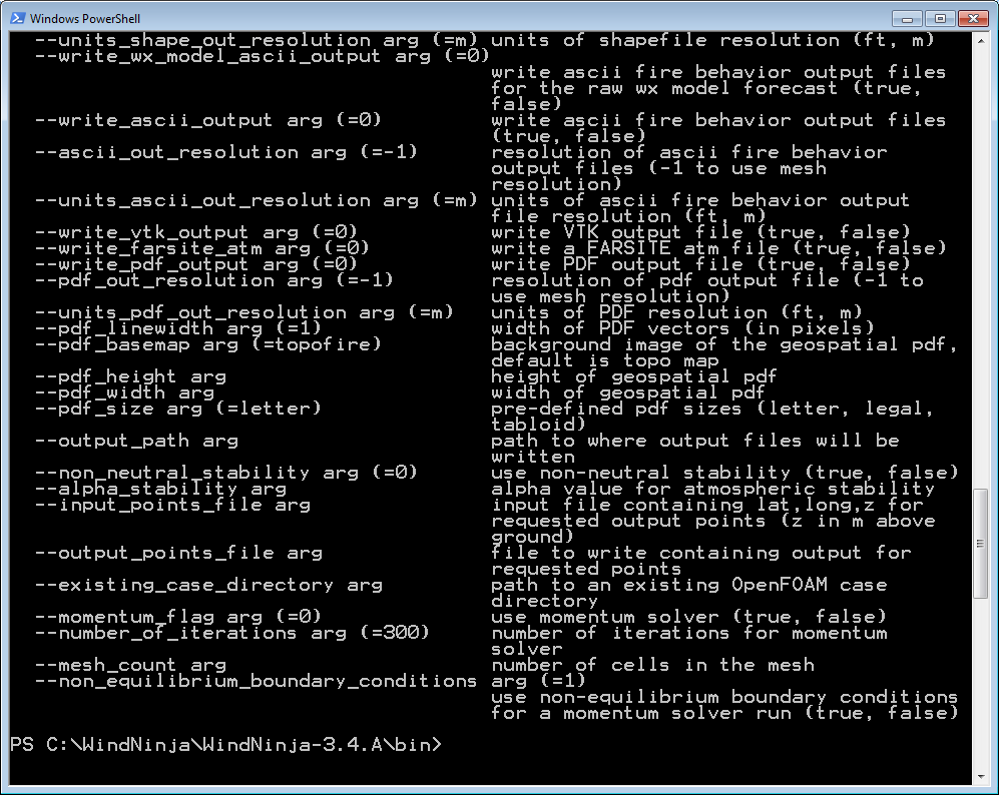
\includegraphics[scale=0.6]{cli-1}
\end{figure}

Options can be used in any order.  Each option has an associated value that can be a string, integer, or float value depending on the option.  Some of the options have a default value that is used if the option is not specified.  The default value is shown in parenthesis (for example,  the \texttt{--num\_threads} option shown above is defaulted to 1 thread).

Depending on the type of run you are trying to do, certain options are required and some are mutually exclusive (ie. can't both be specified at the same time).  If you specify two mutually exclusive options, or don't specify a required option, a message with information on what you did wrong should be shown.  There are too many possible combinations of options to describe here.  Instead, some example configuration files have been included with the installation to show which options to specify for common types of runs.  We recommend starting with one of these example configuration files and modifying them for your purpose.
\newpage
\section*{Starting a run using the terminal}
The terminal can be used to start a run by simply typing “WindNinja\_cli” followed by the option/value pairs separated by a space or “=” like this:
\begin{itemize}
\item[] \texttt{WindNinja\_cli --num\_threads 4 --vegetation=trees} ...etc...
\end{itemize}

\section*{Starting a run using a configuration file}
The configuration files are just text files that list the options and associated values.  The example configuration files provided with the normal WindNinja installation are located in the installation's \say{\textit{etc/windninja/example-files}} directory.  The files are:
\begin{itemize}
\item[] \texttt{cli\_domainAverage.cfg}
\item[] \texttt{cli\_domainAverage\_diurnal.cfg}
\item[] \texttt{cli\_momentumSolver\_diurnal.cfg}
\item[] \texttt{cli\_pointInitialization\_diurnal.cfg}
\item[] \texttt{cli\_wxModelInitialization\_diurnal.cfg}
\end{itemize}

The filenames give insight into what sort of WindNinja run the configuration file does.  For example, the “cli\_wxModelInitialization\_diurnal.cfg” file does a weather forecast model initialized simulation with diurnal flow turned on.  You can open each file to see additional comments describing what the run is doing.  The format of a configuration file is as follows:
\begin{itemize}
\item \say{\texttt{\#}} denotes a comment (to the end of the line)
\item Setting an option is like this:  \texttt{option\_name  =  option\_value}\newline
Note that the \say{\texttt{--}} is not used in the option name in a configuration file.

\end{itemize}

The contents of a configuration file are shown below:
\newpage
\begin{itemize}

\begin{ttfamily}
\item[]
\# \\
\#	This is an example command line interface (cli) configuration file. \\
\#	 \\
\#	This particular file illustrates the necessary options settings to \\
\#	do a weather forecast model initialization run with diurnal winds. \\
\#	The weather model is downloaded via the Internet.  The mesh is set \\
\#	to a specified resolution of 250 meters. \\
\# \\
num\_threads				=	12 \\
elevation\_file				=	C:/XXXX/missoula\_valley.tif \\
initialization\_method			=	wxModelInitialization \\
time\_zone					=	America/Denver \\
wx\_model\_type				=	NCEP-NAM-12km-SURFACE\\ 
forecast\_duration			=	100 \\
output\_wind\_height			=	20.0 \\
units\_output\_wind\_height		=	ft \\
vegetation				=	trees \\
diurnal\_winds				=	true\\ 
mesh\_resolution				=	250.0 \\
units\_mesh\_resolution			=	m \\
write\_goog\_output			=	true \\
write\_shapefile\_output			=	true\\ 
write\_ascii\_output			=	true \\
write\_farsite\_atm			=	true \\
write\_wx\_model\_goog\_output		=	true\\ 
write\_wx\_model\_shapefile\_output	=	true \\
write\_wx\_model\_ascii\_output		=	true\\
\end{ttfamily}

\end{itemize}

To run this particular configuration file, you would just type:

\begin{itemize}
\item[] \texttt{WindNinja\_cli C:/XXXX/cli\_wxModelInitialization\_diurnal.cfg}
\end{itemize}

where \say{\texttt{XXXX}} represents the rest of the path to the file.

\section*{Starting a run by specifying options from both the terminal and a configuration file}

A very useful feature of the WindNinja cli is that you can specify options from both the terminal and a configuration file at the same time.  One way to use this feature would be to put the more \say{general} options in a configuration file, but then specify  other more specific options for the run via the terminal.  If the same option is specified in both the terminal and the configuration file, the terminal value is used.

As an example of this, you could use the configuration file shown above but “override” the elevation file, vegetation, and number of threads options by typing this:

\begin{itemize}
\item[] \texttt{WindNinja\_cli C:/XXXX/cli\_wxModelInitialization\_diurnal.cfg  --elevation\_file C:/XXXX/canyon\_fire.asc --vegetation grass --num\_threads 4}
\end{itemize}

%This isn't included anymore with the default Windows Installation
%commenting out for now
%\section*{Response files}
%Some operating systems (such as older UNIX systems and certain Windows variants)[\href{https://gcc.gnu.org/wiki/Response_Files}{1}] have very low limits of the command line length. One common way to work around those limitations is using response files (instead of configuration files). A response file is just a configuration file which uses the same syntax as the command line (rather than the configuration file syntax described above). If the command line specifies a name of response file to use, it's loaded and parsed in addition to the command line.  We recommend using a configuration file rather than a response file simply because the syntax is more readable and comments are allowed.  The response file method is provided for rare situations where using it might be necessary.
%
%An example response file is located in the installation's “example-files” directory called:
%\begin{itemize}
%\item[] \texttt{cli\_domainAverage\_diurnal.rsp}
%\end{itemize}
%
%To run this response file, you would just type:
%\begin{itemize}
%\item[] \texttt{WindNinja\_cli @C:/XXXX/cli\_wxModelInitialization\_diurnal.rsp}
%\end{itemize}
%
%where \say{\texttt{XXXX}} represents the rest of the path to the file.
%Notice the \say{\texttt{@}} character preceding the response file name, which identifies it as a response file.

\end{document}